\documentclass[aip,amsmath, reprint, author-year,nobalancelastpage]{revtex4-1}
\usepackage{url}
\usepackage[utf8]{inputenc}

\usepackage{graphicx} % for graphics
\usepackage{float}
\usepackage{hyperref}
%\usepackage{listings} % for code listtings
%\usepackage{color}

%\setcitestyle{round, author-year}

\setcounter{page}{1}

%\bibliographystyle{aipauth4-1.bst}


\begin{document}

\begin{abstract}
Everything needed 
\end{abstract}

\title{Further investigations - DRAFT}
\author{Andreas Bruun Okholm, s082562\\
Mathias Rask Møller, s082536 }
\affiliation{Technical University of Denmark}
 
\date{\today}
\maketitle


Using todays technology, generalisation of PC data upon request from the user I feasible. A proposed technical setup is described in \cite{OkholmRask******* Techpaper}.

apply tolerance, By looking at normalised data of the variance of products of the same material and process, it is possible to find a suitable tolerance
improvement per rework
material selection

\emph{What you measure and index is what you can analyse from.}
The index and type of samples limits the possible conclusions, which can be mades when extracting the data.  (If the goal is to understand the long term process capability impact of an injection mould process it is either necessary to have measurement sets from many products at different stages of their lifespan or multiple measurements through the lifespan of a couple of products.   

Initiating PCG is a tough process. 
The reward for doing robust design engineering is long reach
The reward for using PCDB or robust design in general to make changes in early design is a long term and might only benefit the company and not feedback to the designers compared the reward for the hero in production solving the expensive errors in design.

Implementing GPC requires a change
	economical barrier
		big company
			incement from quality department
			gain: 	knowledge of own PC
					high precision data
					Extensive knowledge on causes and problem
			Loss:
		cross companies
			diverse data
			gain:		Alot of data
					knowledge of processes and material outside your field
					knowledge of possible to achieve in industry
					Index storing of own data and partially analysed
			loss:		Industry espionage concerns
					loss of information due to anonymity

proto running at a university, unbiased.


\begin{verbatim}
ITG
Concentricity
Ca (bias,std)
Cp
circularity

ITG .. batch
ITG .. dimensions
ITG .. mold
ITG .. mold lines
ITG .. inside/outside

Ca .. radii vs. postions
Ca .. mold lines
 
CaSpec .. inside

circ .. dimension
circ .. inside/outside

conc .. dimension

ITG .. ITG spec

bias .. std

measurement tech
ITG .. ITG china

Standard deviation correction factor.
\end{verbatim}


\begin{verbatim}
ONE PAGER til ccplast

ITG .. ITG spec 
PCSL table for hver måling.
ITG table for hver måling.

ITG .. hole and shaft

ITG .. Dimension

bias vs. std. + cpk lines


\end{verbatim}


The confidence interval of the population standard deviation is greatly effected by the sample size.  The confidence limits are given by

\begin{equation}
\left[ \sqrt{\frac{(n-1) \hat{\sigma}^2 }{\chi^2_{\alpha/2,n-1}}},  \sqrt{\frac{(n-1) \hat{\sigma}^2 }{\chi^2_{1-\alpha/2,n-1}}} \  \right]
\end{equation}
where $\chi^2$ is the chi-squared distribution, n is sample size and $\alpha$ is the significance level. The confidence limits are shown in Figure \ref{fig:std_uncertainty}. Even for samples sizes of 30 there still exist a quite large uncertainty of the standard deviation, which also directly effect the process capability indices and the calculated PCSL. 


\section{discarded material }

\newpage
\subsection{Uncertainty of standard deviation}

\begin{figure}[H]
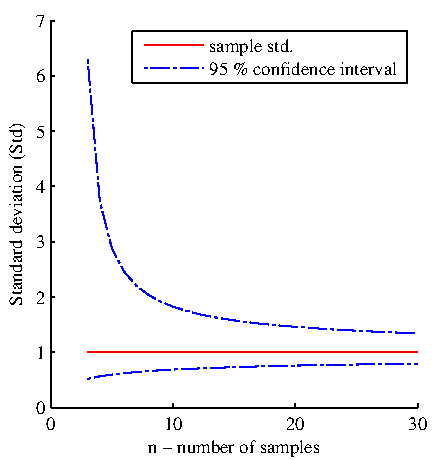
\includegraphics{stats_std_confidence.pdf}
\caption{\label{fig:std_uncertainty}Confidence interval for the population standard deviation compared to a sample standard deviation as a function of sample size. The gained certainty per measurement is best for low sample sizes.}
\end{figure}

Figure \ref{fig:std_uncertainty} shows the analytical solution to a uncertainty of a standard deviation of a sample compared to the deviation of the population as a function of sample size. 

\newpage
\subsection{Uncertainty of mean shift }
\begin{figure}[H]
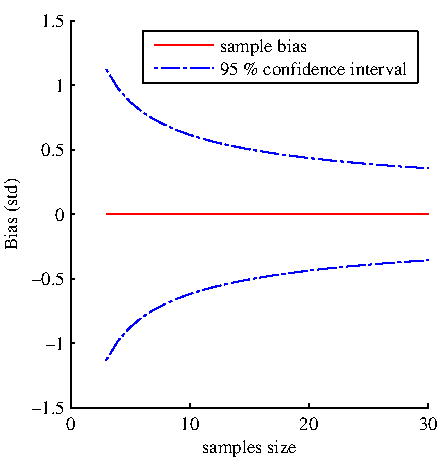
\includegraphics{stats_bias_confidence.pdf}
\caption{\label{fig:bia_uncertainty}Confidence interval for the population bias as a function of sample size. The gained certainty per measurement is best for low sample sizes.}
\end{figure}

Figure \ref{fig:bia_uncertainty} shows the analytical solution to uncertainty of mean shift. 


\newpage
\subsection{Monte Carlo}
\begin{figure}[H]
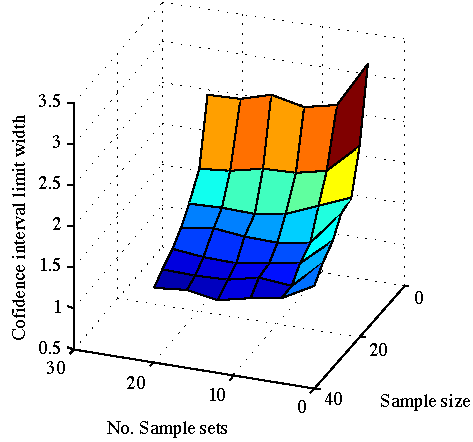
\includegraphics{CLW90_surf.pdf}
\caption{\label{fig:CLW90_surf} Confidence interval width at 90\% probability as a function of sample size and number of measuments.}
\end{figure}

Figure \ref{fig:CLW90_surf} shows a surf representation of confidence interval width at $ 90 \%$ probability. The sample size has very little influence for sample of more than 12 samples. 

\newpage

\subsection{Cofidence interval width function}
\begin{figure}[H]
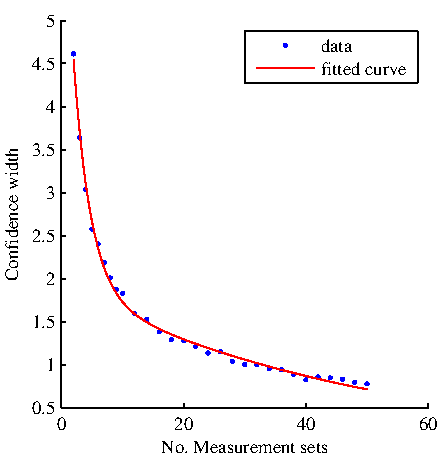
\includegraphics{regresion_sample_sets.pdf}
\caption{\label{fig:reg_sample} Confidence interval width as a function for number of measurement sets.   }
\end{figure}



\newpage

\subsection{Normal distribution of data}
\begin{figure}[H]
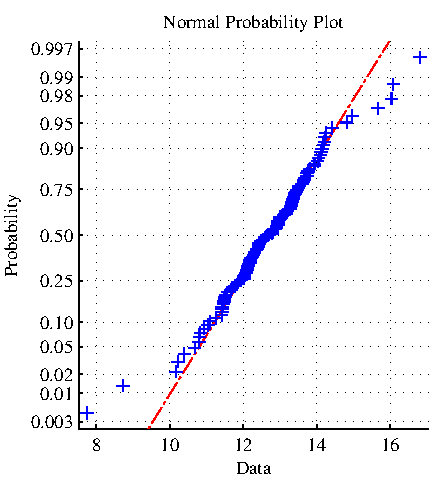
\includegraphics{Normal_plot.pdf}
\caption{\label{fig:normplot} Normality investigation of IT-grades of Vaavud Windmeter data   }
\end{figure}

Figure \ref{fig:normplot} shows a normal distribution plot. The Normalised data from the windmeter measurement sets is close to the line. A Normal distribution is a good fit.


\newpage

\subsection{IT-grade verification}
\begin{figure}[H]
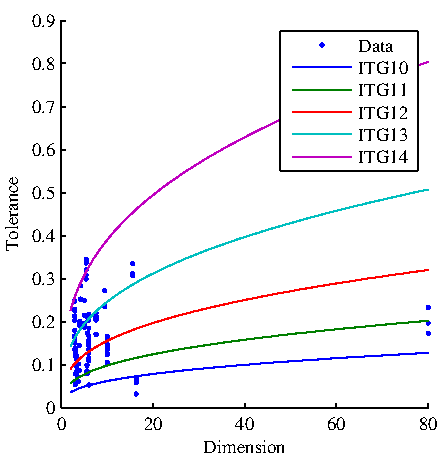
\includegraphics{DimTol.pdf}
\caption{\label{fig:dimtol} Data from windmeter plotted together with the lines for the IT-grade. }
\end{figure}

The plot is inconclusive. There is not enough data for verify the IT-grade scales.


\newpage

\subsection{Bias investigation}
\begin{figure}[H]
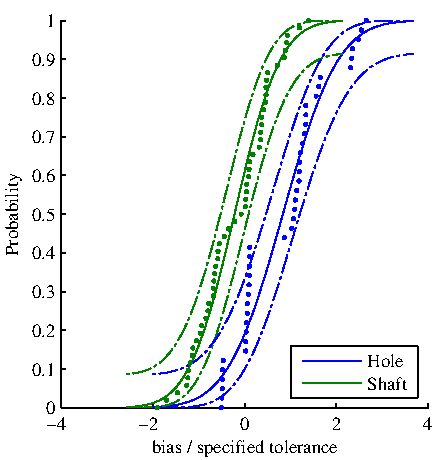
\includegraphics{CA_inside.pdf}
\caption{\label{fig:CA_inside} Normalised bias accumulated frequency plot for measurement on the inside and outside measurements of features}
\end{figure}

Figure \ref{fig:CA_inside} shows that there is a significant difference on bias of measurements of hole and shafts. Holes are made a full tolerance length too big. Shafts are generally made on target.

This is probably done to ensure functionallity. Wear on the mold will make holes smaller and shafts bigger. 


\newpage

\subsection{Material selection}
\begin{figure}[H]
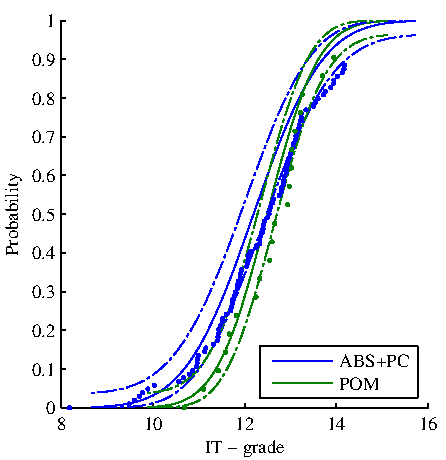
\includegraphics{ITG_material.pdf}
\caption{\label{fig:CA_inside} IT-grade accumulated frequency plot for measurements of different materials}
\end{figure}

POM seems to be prefoming more consistently than ABS.

This Comparison gives a overview of what process capabilities are in the different materials.

But since this only represents 1 sample of each material, this is not usable. Too little data. 
The samples also represent the difference between single and multi cavity mods, and different mold material type. 

	
\newpage

\subsection{Tolerance specification}
\begin{figure}[H]
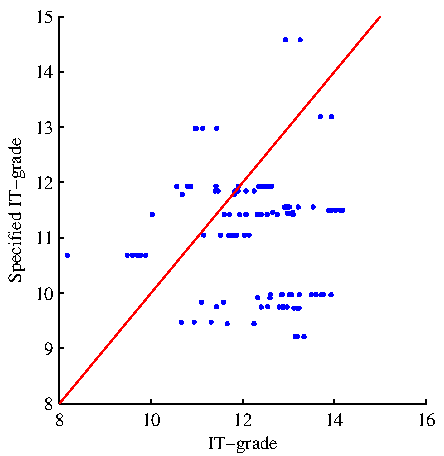
\includegraphics{ITG_ITGSpec.pdf}
\caption{\label{fig:ITG_ITGSpec} IT-grade and specified tolerances IT-grade plotted.}
\end{figure}

Points above the line exceeds the specified tolerance. 

\newpage

\subsection{Dimesion Capability}
\begin{figure}[H]
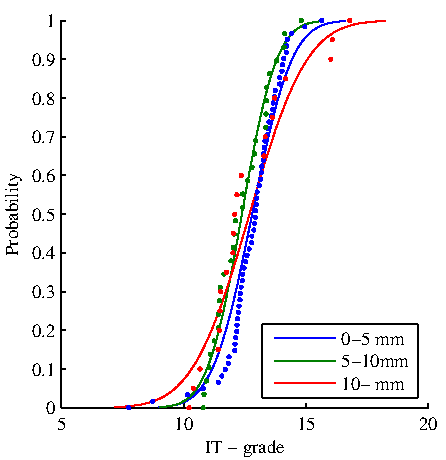
\includegraphics{ITG_DimSort.pdf}
\caption{\label{fig:ITG_DimSort} IT-grade plotted for features of dimension intervals  }
\end{figure}

Large geometries deviates more. 
Data has been aggregated: Measurement of identical feature and color batch are aggregated.

\newpage

\subsection{Measurement technology}
\begin{figure}[H]
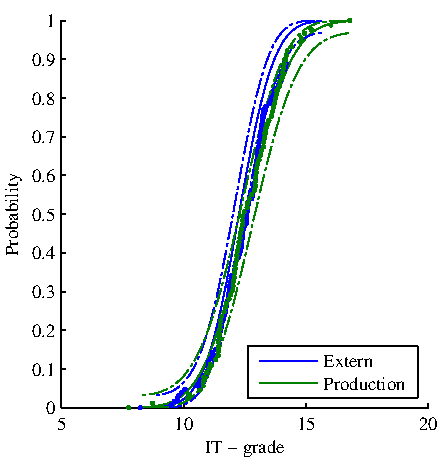
\includegraphics{ITG_china.pdf}
\caption{\label{fig:ITG_china} IT-grade plotted Measured by production in china and by MetroloTechnological Institute  }
\end{figure}

Large geometries deviates more. 
Data has been aggregated: Measurement of identical feature and color batch are aggregated.

\newpage

\subsection{Dimesion Capability}
\begin{figure}[H]
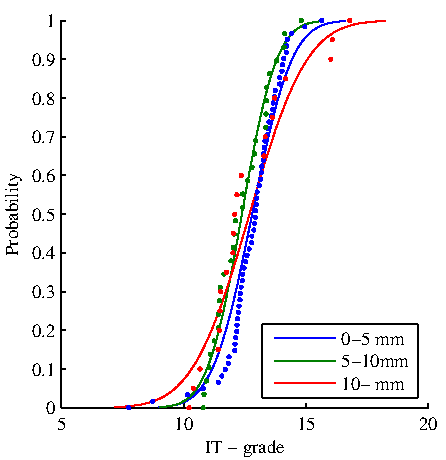
\includegraphics{ITG_DimSort.pdf}
\caption{\label{fig:ITG_DimSort} IT-grade plotted for features of dimension intervals  }
\end{figure}

Large geometries deviates more. 
Data has been aggregated: Measurement of identical feature and color batch are aggregated.


\end{document}